\documentclass[letterpaper, 10 pt, conference]{ieeeconf}
\IEEEoverridecommandlockouts
\overrideIEEEmargins

\usepackage{graphicx}
\usepackage[T1]{fontenc}   % needed for accents such as \k{a} in bib entries
% ieeeconf.cls defines \proof; amsthm redefines it -> "already defined".
\let\proof\relax
\let\endproof\relax
\usepackage{amsmath, amssymb, amsfonts, amsthm}
\usepackage[dvipsnames]{xcolor}
\usepackage{array, tabularx, booktabs, multirow, makecell}
\usepackage{algorithm, algpseudocode}
\usepackage{cleveref}

\graphicspath{{figures/}}

\newtheorem{theorem}{Theorem}
\newtheorem{proposition}{Proposition}
\newtheorem{lemma}{Lemma}
\theoremstyle{remark}
\newtheorem*{note}{Note}

\crefname{figure}{Fig.}{Fig.}
\Crefname{figure}{Figure}{Figures}
\Crefname{equation}{Equation}{Equations}
\crefname{theorem}{Theorem}{Theorems}
\crefname{section}{Section}{Sections}
\crefname{proposition}{Proposition}{Propositions}
\crefname{algorithm}{Algorithm}{Algorithm}
\crefname{table}{Table}{Tables}

% ---------------------------------------------------------------------------
% \todo{...} — inline red note for drafting. Swap the two definitions below to
% hide every note at once for a submission build.
% ---------------------------------------------------------------------------
\newcommand{\todo}[1]{\textcolor{red}{\bfseries [TODO: #1]}}
%\newcommand{\todo}[1]{}

% ---------------------------------------------------------------------------
% DRAFT SCAFFOLDING — space budget. Delete this whole block, every \lipsum,
% every \figbox and every \budget before submission.
%   \budget{...}            blue marker: target length for the section it heads
%   \lipsum[a-b]            filler prose, ~100 words per paragraph
%   \figbox{<h>}{<label>}   grey box the height the final figure will occupy
%   \nocite{*}              pulls all of refs.bib in so the bibliography has
%                           real height (final list will be ~2x this long)
% Calibrated so the whole skeleton lands on exactly 8 pages. As you replace a
% \lipsum with prose, the page count tells you whether you are over or under.
% ---------------------------------------------------------------------------
\usepackage{lipsum}
\newcommand{\budget}[1]{\textcolor{RoyalBlue}{\bfseries [BUDGET: #1]}}
\newcommand{\figbox}[2]{%
  \fcolorbox{gray}{gray!12}{\parbox[c][#1][c]{\dimexpr\linewidth-2\fboxsep-2\fboxrule\relax}%
    {\centering\ttfamily\footnotesize #2}}}

\title{\LARGE \bf A Multi-Agent Path Planner for Escorted Navigation in GPS-Denied Environments}

% ICRA 2027 uses double-anonymous review: the submitted PDF must carry no
% author names or affiliations. Restore the real list after acceptance.
\author{Anonymous Authors}

\begin{document}

\maketitle
\thispagestyle{empty}
\pagestyle{empty}

\begin{abstract}
Centralized multi-agent path planning with cooperative localization in GPS-denied environments is generally computationally 
intractable when formulated in full belief space due to tightly coupled uncertainty dynamics. Prior work either approximates belief dynamics
or restricts inter-agent coupling. We study a multi-agent planning problem in which a primary agent must reach a goal in minimum time 
subject to a chance-constrained collision-avoidance requirement and a terminal bound on localization uncertainty. We obtain a tractable surrogate
of the underlying belief-space problem by optimizing over the mean-state trajectories of all agents and propagating covariance for terminal constraint evaluation only. 
We propose a discrete-to-continuous pipeline combining hexagonal-grid joint search with spline-based trajectory refinement. 
Across 50 randomized scenarios, when the terminal uncertainty constraint is 50\% of the terminal uncertainty of a reference lone primary agent plan, our planner
finds solutions in 80\% of the scenarios against 54\% for the strongest baseline. We validate these results through the marine robotics simulator HoloOcean~\cite{potokar2022holoocean} and show that
the generated paths satisfy the collision constraint in 100\% and the terminal uncertainty bound in 93\% of closed-loop Monte Carlo trials.

\end{abstract}

% ===========================================================================
\section{INTRODUCTION}
% ===========================================================================
%\budget{$\approx$550 words, 0.7 page incl.\ Fig.~1}

\begin{figure}[t]
  \centering
  \figbox{6.5cm}{Fig.~1 --- overview: domain (GPS-denied, escorted primary), the
    discrete-to-continuous pipeline, and the contribution in one frame}
  \caption{Overview. A primary agent (\todo{color}) must reach the goal under a
    terminal localization bound while support agents act as mobile landmarks.
    Left: the heading-aware hexagonal graph and the joint discrete search.
    Right: the continuous B-spline refinement of the same plan.
    \todo{write real caption}}
  \label{fig:overview}
\end{figure}
In environments where GPS signal is unreliable, such as underwater, or in regions subject to spoofing or jamming, agents must rely on other forms of information
for localization via GPS-denied solutions. In GPS-denied environments, autonomous agents struggle with state uncertainty due to inertial measurement unit (IMU)
drift. As the estimation error accumulates, an agent's pose uncertainty can grow to a point where waypoint tracking degrades and mission objectives are compromised.
Common planning strategies ameliorate this by biasing trajectories toward informative landmarks and introducing cooperating agents to utilize inter-agent measurements for 
cooperative localization~\cite{roumeliotis2002dist,bahr2009coop}. Consequently, trajectory planning must account for uncertainty propagation when estimation error impedes task performance. While
belief-space planning provides a principled formulation for uncertainty-aware decision making, it is typically intractable in multi-agent settings due to the dimensionality of coupled
belief dynamics~\cite{kaelbling1998pomdp,platt2010belief}. This motivates surrogate formulations that optimize mean trajectories while propagating uncertainty only for constraint evaluation.

In this work, we consider a centralized multi-agent planning problem in which a primary agent must reach a goal in minimum time while subjected to a chance-constrained collision-avoidance 
requirement and a terminal bound on localization uncertainty.

We compute a coordinated discrete plan over a joint state space that captures motion constraints and inter-agent ranging capabilities. This solution is then lifted into
continuous space and refined into smooth, dynamically feasible trajectories that satisfy kinematic constraints.

Our contributions are as follows:
\begin{enumerate}
  \item A formulation of centralized multi-agent path planning with cooperative
    localization (MAPP-CL) in the presence of obstacles, in which support
    agents are routed jointly with a primary agent subject to a terminal
    localization bound and chance-constrained collision avoidance under both
    agent and obstacle uncertainty.
  \item A discrete-to-continuous planner, a joint search over a heading-aware
    hexagonal lattice followed by B-spline refinement, that enforces the
    curvature, collision, and terminal-uncertainty constraints in both stages.
  \item A benchmark of 50 randomized scenarios against four baselines adapted
    from adjacent literature, on which the planner solves 80\% of scenarios at
    the 50\% constraint level against 54\% for the strongest baseline.
  \item Closed-loop Monte Carlo validation in HoloOcean with an independent
    factor-graph estimator, showing that the collision constraint holds in 100\% and the terminal
    uncertainty bound in 93\% of trials.
\end{enumerate}

In the following sections, we formalize the problem, describe the discrete and continuous planning stages and evaluate our approach in a simulated GPS-denied environment.


% ===========================================================================
\section{RELATED WORK}
\label{sec:related}
% ===========================================================================
Planning under uncertainty is naturally posed as a partially observable Markov
decision process, which is intractable in general \cite{kaelbling1998pomdp}.
Belief-space planners make the problem tractable by restricting beliefs to
Gaussians and propagating them along candidate trajectories, either over a
roadmap \cite{prentice2009brm}, a tree \cite{bry2011rrbt}, or a locally
optimized path \cite{vandenberg2011lqgmp}, and they typically assume that the
most likely observation is received \cite{platt2010belief}. These methods plan
for a single agent. With several agents the belief includes every agent's
state, the agents are coupled through inter-agent measurements, and the search
space grows exponentially with the size of the team.

Cooperative localization lets agents share position estimates to reduce
dead-reckoning drift \cite{roumeliotis2002dist,bahr2009coop}, and it is a
standard tool in underwater navigation, where GPS is unavailable below the
surface \cite{paull2014auv}. Because cooperating agents share measurement
history, naive fusion double counts information, and covariance intersection
\cite{julier1997cov} is the usual remedy for fusion under unknown correlation
\cite{carrillo2013ci}. Planning with cooperative localization in the loop is
more recent. Theurkauf et al. \cite{theurkauf2025coop} grow a sampling-based
tree over the joint belief of a team and bias it toward configurations that
keep the agents in range of one another, and Liu et al. \cite{liu2026risk}
plan risk-aware trajectories for underwater teams that localize cooperatively.
Our work differs in that the support agents have no goals of their own and are
routed only to meet the primary's terminal bound, and in that the joint search
is exhaustive on a lattice rather than sampled.

Multi-agent path finding solves the discrete coordination problem exactly, for
example with conflict-based search \cite{sharon2021cbs}, or approximately by
planning the agents one at a time in priority order
\cite{erdmann1987multiple,silver2005cooperative}. Both treat agent positions
as known and do not model localization. Our sequential baseline adapts
prioritized planning to the escort problem.

Grid-based search followed by continuous refinement is a common way to satisfy
kinematic constraints. Hexagonal grids offer uniform neighbour spacing and
less directional bias than square grids \cite{duszak2021hexgrid}, and
B-splines give smooth trajectories with local control whose curvature can be
bounded \cite{feng2024bsrrt,karaman2011optimal}. Obstacle avoidance under
position uncertainty follows the chance-constrained formulation of Blackmore
et al. \cite{blackmore2011chance}, and we bound each spline segment by its
MINVO hull \cite{tordesillas2022minvo} so that the constraint is linear in
the control points.

% ===========================================================================
\section{PROBLEM FORMULATION}
\label{sec:pf}
% ===========================================================================
Let $\mathcal{I} = \{1,2,\dots,P\}$ denote a team of $P$ agents, where agent $i=1$
is the primary agent tasked with reaching a goal location $G\in\mathbb{R}^2$.
All other agents $2,\dots,P$ are support agents whose sole task is to assist the
primary agent's localization. All agents move at a common constant speed $v$,
so minimizing time is equivalent to minimizing trajectory length, and we use
arc length $s = vt$ as a shared clock throughout. The environment contains $M$
static convex obstacles $\mathcal{O}_1,\dots,\mathcal{O}_M$, each defined as an
intersection of half-planes $a_j^{\top}x \le b_j$ with unit outward normals
$a_j$ and offsets $b_j$, and each located only up to a covariance $\Sigma_o$.
The environment also contains a set $\mathcal{L}$ of landmarks with known
positions $\ell\in\mathbb{R}^2$ and positional uncertainty $\Sigma_\ell$.

\subsection{Decision Variables}

We optimize over mean-state trajectories only. The decision variables are the
heading profile $\theta_i(s)$ of every agent and the primary's path length
$S_1$. Positions follow from the headings at the arc samples
$s_k = k\,\Delta s$ through
\begin{equation}
  x_i(s_{k+1}) = x_i(s_k) + \Delta s
  \begin{bmatrix} \cos\theta_i(s_k) \\ \sin\theta_i(s_k) \end{bmatrix}.
  \label{eq:dyn}
\end{equation}

\subsection{Covariance Propagation}

Let $\Sigma_i(s)$ denote the $2\times2$ position covariance of agent $i$.
Covariance is not a decision variable. It is propagated along the mean
trajectories and used only to evaluate constraints. Between measurements the
agents dead-reckon, and we model the resulting drift as process noise whose
variance grows linearly with the distance travelled and is larger along the
direction of travel than across it:
\begin{equation}
  \Sigma_i^{-}(s_{k+1}) = \Sigma_i(s_k) + Q\big(\theta_i(s_k)\big)\,\Delta s,
  \label{eq:prop}
\end{equation}
where $Q(\theta) = R(\theta)\,\mathrm{diag}(q_\parallel, q_\perp)\,R(\theta)^{\!\top}$,
$R(\theta)$ is the planar rotation matrix, and $q_\parallel \ge q_\perp$ are
the along-track and cross-track noise intensities.

\subsection{Landmark Measurements}

A landmark $\ell$ provides a range-bearing measurement whose quality decays
smoothly with the distance $d_{i\ell} = \lVert x_i - \ell \rVert$ through the
logistic taper
\begin{equation}
  q_{i\ell} = \frac{1}{1 + \exp\!\big((d_{i\ell} - r_v)/w_v\big)},
  \label{eq:taper}
\end{equation}
which is close to one inside the visibility range $r_v$ and rolls off over a
width $w_v$. There is no hard sensing cutoff. Every landmark contributes
information weighted by its quality, and the posterior covariance follows the
information form of the Kalman update for a direct position measurement,
which for $H = I$ is identical to the Joseph form:
\begin{equation}
  \Sigma_i(s_k) = \Big( \Sigma_i^{-}(s_k)^{-1}
  + \sum_{\ell \in \mathcal{L}} q_{i\ell}\,\big(S_{i\ell} + \Sigma_\ell\big)^{-1} \Big)^{-1},
  \label{eq:lm}
\end{equation}
where $S_{i\ell} = R(\beta_{i\ell})\,\mathrm{diag}(\sigma_r^2, \sigma_b^2)\,R(\beta_{i\ell})^{\!\top}$
is the range-bearing sensor noise rotated to the line-of-sight bearing
$\beta_{i\ell}$.

\subsection{Inter-Agent Fusion}

Agents exchange position estimates at fixed arc-length intervals $\Lambda$.
The estimates of cooperating agents share history, so adding their
information directly would double count it. We therefore fuse with covariance
intersection \cite{julier1997cov}, which remains consistent under unknown
cross-correlation. When agents $i$ and $j$ communicate at separation
$d_{ij}$, agent $i$ receives the transferred estimate
$P_{j \to i} = (\Sigma_j + R_c)/w_{ij}$, where $R_c = \sigma_c^2 I$ is the
communication noise and $w_{ij}$ is a logistic taper of the form
\eqref{eq:taper} with half weight at the communication range $r_c$. The
update is
\begin{equation}
  \Sigma_i^{+} = \Big( \omega\,\Sigma_i^{-1} + (1-\omega)\,P_{j \to i}^{-1} \Big)^{-1},
  \label{eq:ci}
\end{equation}
with $\omega \in [0,1]$ chosen to minimize $\det\Sigma_i^{+}$, and agent $j$
is updated in the same way. As $w_{ij} \to 0$ the transferred information
vanishes, so agents that are far apart do not fuse.

\subsection{Optimization Problem}

The planning problem collects the objective and all constraints as
\begin{subequations}
\label{eq:opt}
\begin{align}
  & \min_{\{\theta_i(\cdot)\},\, S_1}\;\; S_1 \nonumber \\
  & \mathrm{s.t.}\;\;
    \det\big(\Sigma_1(S_1)\big)^{1/4} \le \bar{u}, \label{eq:term} \\
  & a_j^{\top} x_i(s) \ge b_j + r_a
      + z_\delta \sqrt{a_j^{\top}\big(\Sigma_i(s) + \Sigma_o\big)a_j},
      \label{eq:cc} \\
  & |\kappa_i(s)| \le 1/r_{\min}, \label{eq:kin} \\
  & x_i(0) = x_i^0,\;\; \Sigma_i(0) = \Sigma^0,\;\; x_1(S_1) = G.
      \label{eq:bc}
\end{align}
\end{subequations}

\textbf{Terminal uncertainty \eqref{eq:term}.} The primary must arrive with
bounded localization uncertainty. The quantity $\det(\Sigma)^{1/4}$ equals
the standard deviation $\sigma$ for an isotropic covariance $\sigma^2 I$, so
the bound $\bar{u}$ is expressed in metres.

\textbf{Obstacle avoidance \eqref{eq:cc}.} Every agent must clear every
obstacle with probability at least $1-\delta$ at every instant. For each
agent $i$, obstacle $o$, and arc position $s$, the constraint must hold for
at least one face $j$ of $\mathcal{O}_o$. The mean position then lies outside
that face with a margin that covers the vehicle radius $r_a$ and both the
agent's and the obstacle's positional uncertainty, where
$z_\delta = \Phi^{-1}(1-\delta)$ and $\Phi$ is the standard normal
distribution function \cite{blackmore2011chance}. A union bound over the
$PM$ agent-obstacle pairs bounds the instantaneous probability of any
collision by $\Delta = PM\delta$.

\textbf{Kinematics \eqref{eq:kin}.} Each trajectory respects the vehicles'
minimum turn radius $r_{\min}$, where $\kappa_i = \mathrm{d}\theta_i/\mathrm{d}s$
is the path curvature.

\textbf{Boundary conditions \eqref{eq:bc}.} All agents start from known
positions with a common prior covariance, and the primary must end at the
goal.

The belief dynamics do not appear as constraints. $\Sigma_i(s)$ is a
deterministic function of the decision variables through
\eqref{eq:dyn}--\eqref{eq:ci}, and this dependence is left implicit in
\eqref{eq:opt}. The agents are coupled only through the fusion step
\eqref{eq:ci}. The supports' trajectories enter the problem only by shaping
the primary's covariance, and this coupling is what makes the problem a
joint one.

% ===========================================================================
\section{METHOD}
\label{sec:method}
% ===========================================================================
Our planner solves \eqref{eq:opt} in two stages. A joint A* search over a
heading-aware hexagonal lattice produces a coordinated discrete plan for all
agents, and a continuous optimization refines that plan into smooth B-spline
trajectories that satisfy the curvature, collision, and terminal uncertainty
constraints. Algorithm~\ref{alg:joint} summarizes the full pipeline.

\subsection{Heading-Aware Hexagonal Graph}

The environment is covered by a corridor of hexagonal cells of width
$w_{\mathrm{hex}}$ around the line from start to goal
\cite{duszak2021hexgrid}. A graph node pairs a cell with one of six headings
spaced $60^\circ$ apart, and exactly three moves leave each node: continue
straight, or turn by $\pm 60^\circ$ and step into the cell faced by the new
heading. The heading therefore changes by at most $60^\circ$ per cell
traversed, which serves as the graph-level counterpart of the curvature bound
\eqref{eq:kin}. Landmarks are appended as sensor nodes that carry no edges
and enter the search only through the measurement update \eqref{eq:lm}. A
goal node absorbs all six headings of the goal cell, so the arrival heading
is unconstrained. Obstacles do not remove cells from the graph. They act on
the beliefs during the search described next. Finally, all-pairs
shortest-path distances are precomputed on the graph and serve as the search
heuristic.

\subsection{Joint Discrete Search}

The first stage searches for a resolution-constrained solution of
\eqref{eq:opt} with an A*-style search \cite{hart1968astar} over the joint
state of the team. A search state stores, for every agent, its graph node,
its covariance, and the arc distance it has travelled. Each expansion
advances every agent by one edge, so the successors of a state are the
Cartesian product of the agents' three moves. The accumulated cost $g$ is the
primary's arc distance alone, and states are expanded in order of
$f = g + (1+\varepsilon)\,h$, where $h$ is the precomputed shortest-path
distance from the primary's node to the goal. Support agents contribute no
heuristic cost, so $h$ is an admissible lower bound and the search with
$\varepsilon = 0$ is admissible. With $\varepsilon > 0$ the search becomes a
weighted A* \cite{pohl1970weighted} that trades a factor of
$(1+\varepsilon)$ on the seed length for fewer expansions. Ties are broken
toward lower primary uncertainty and then toward fewer idle supports.

During expansion each agent's covariance is propagated along its edge by
\eqref{eq:prop}--\eqref{eq:lm}, and covariance intersection \eqref{eq:ci} is
applied whenever two agents reach a communication checkpoint at the same arc
distance. A successor is discarded if any agent violates the chance
constraint \eqref{eq:cc} along its edge or if a support travels farther than
the primary. The joint space is kept manageable by Pareto pruning. At each
joint node signature the search keeps a frontier of $(g, \Sigma_1)$ labels
and discards a new label if an existing one has no larger $g$ and a
covariance no larger in the positive semidefinite order. This pruning is
sound because the heuristic is shared at the same node tuple, the primary
path cost of the dominated state cannot be lower, and a covariance that is
larger in the positive semidefinite order cannot become smaller under
further propagation.

The search is anytime with respect to the terminal constraint
\eqref{eq:term}. When a popped state places the primary at the goal and the
spline seed it induces (Sec.~\ref{sec:cont}) clears all obstacles, the state
is returned immediately if \eqref{eq:term} holds. Otherwise the state is
kept as the incumbent if its terminal uncertainty is the lowest seen so far.
If the expansion budget is exhausted, the incumbent is handed to the
continuous stage, which attempts to recover feasibility. Only the terminal
bound is relaxed in this way. Obstacle clearance is never relaxed.

\begin{note}
Six headings quantize direction to within $30^\circ$, so a lattice path that
traces a smooth trajectory is at most $2/\sqrt{3}$ times longer than it. If
\eqref{eq:opt} has a solution whose constraint slacks are strictly positive,
a fine enough lattice therefore contains a feasible seed within that factor
of the optimum, and the admissible search returns a feasible seed no longer
than it. The factor comes from the move set rather than the resolution, and
removing it is the job of the continuous refinement.
\end{note}

\begin{algorithm}[t]
  \caption{Discrete-to-continuous escort planning}
  \label{alg:joint}
  \begin{algorithmic}[1]
    \Require hex graph, start states $\Sigma^0$, goal $G$, bound $\bar{u}$,
      budget $N$
    \State precompute all-pairs graph distances $h(\cdot)$
    \State $\mathit{open} \gets \{\text{joint start}\}$;\quad
      $\mathit{inc} \gets \varnothing$
    \While{$\mathit{open} \neq \varnothing$ and expansions $< N$}
      \State pop state minimizing $f = g + (1+\varepsilon)h$
      \If{primary at goal \textbf{and} seed spline clears obstacles}
        \If{$\det(\Sigma_1)^{1/4} \le \bar{u}$}
          seed $\gets$ state; \textbf{break}
        \ElsIf{lowest terminal uncertainty so far}
          $\mathit{inc} \gets$ state
        \EndIf
      \EndIf
      \ForAll{joint successors (every agent one edge)}
        \State propagate $\Sigma_i$ by \eqref{eq:prop}--\eqref{eq:lm};
          fuse by \eqref{eq:ci}
        \State discard if \eqref{eq:cc} violated or a support outruns
          the primary
        \State insert unless dominated in $(g,\Sigma_1)$ at its signature
      \EndFor
    \EndWhile
    \State \textbf{if} no seed \textbf{then} seed $\gets \mathit{inc}$
      \Comment{least-violating}
    \State $x \gets$ control points of seed splines;\quad
      $\mathit{feas} \gets \min s(x) \ge 0$
    \For{each barrier stage; Adam iterations on $\nabla_x J(x;\mu)$}
      \State accept step iff $J$ decreases and
        ($\neg\mathit{feas}$ \textbf{or} trial feasible)
      \State $\mathit{feas} \gets \mathit{feas} \lor \text{trial feasible}$
        \Comment{latch}
      \State track least-violating / shortest-feasible incumbents
      \State decay $\mu$ only once $\mathit{feas}$
    \EndFor
    \State \Return best incumbent trajectory
  \end{algorithmic}
\end{algorithm}

% Fig.~2 is a two-column float; LaTeX places figure* at the top of the NEXT
% page after its source position, so it is issued here to land on the page
% where Results begins. Move the source if it drifts.
\begin{figure*}[t]
  \centering
  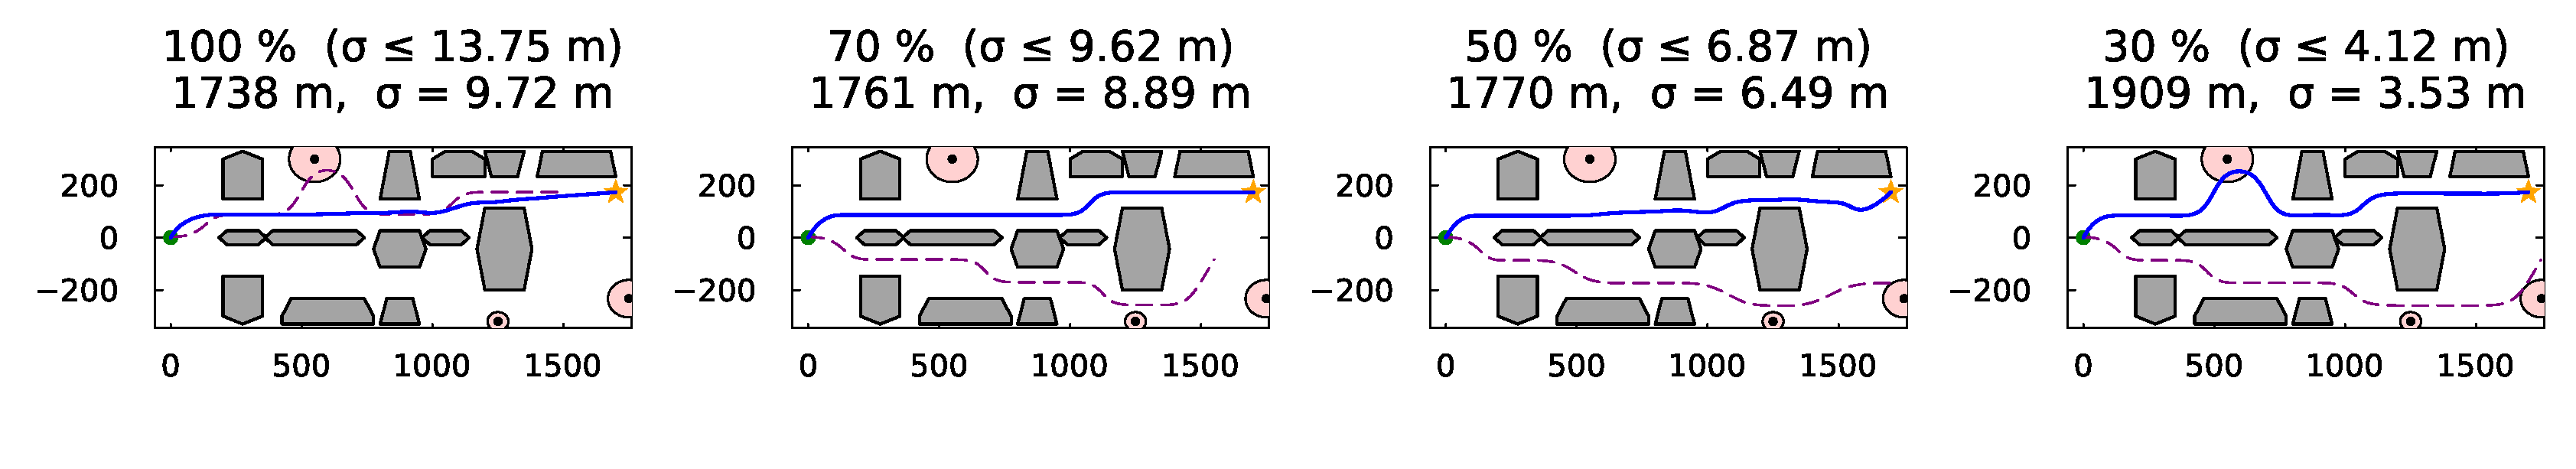
\includegraphics[width=\textwidth]{fig2_ladder_ours_shapes_v14}
  \caption{Constraint ladder on one scenario (1700\,m corridor, 13 obstacles,
    three landmarks, $\varepsilon = 0$, 100\,m lattice). Each panel is our
    planner's solution as the terminal bound tightens from 100\% to 30\% of
    the single-agent reference $U_\mathrm{ref}$. The primary is the solid
    curve and the support the dashed one, landmarks are dots with their map
    covariance, and each title gives the primary's length and terminal
    $\sigma$. At 100\% the support climbs into the upper pocket to sight the
    weak landmark there and rejoins (1738\,m). At 70\% it takes the southern
    lane to a stronger landmark and relays it at half weight (1761\,m). At
    50\% the primary adds one turn before the goal so that the support can
    reach that landmark in time (1770\,m, $\sigma = 6.5$\,m). At 30\% the
    primary itself detours through the obstacle row toward the third landmark
    (1909\,m, $\sigma = 3.5$\,m).}
  \label{fig:ladder}
\end{figure*}

\subsection{Continuous B-Spline Refinement}
\label{sec:cont}

The discrete seed is lifted into continuous space as clamped cubic B-splines
\cite{piegl1997nurbs}, one per agent, whose control points are the centres of
the seed's cells. Support paths are padded to the primary's node count, and
the primary's final control point is pinned to $G$. The decision vector $x$
stacks the free control points: every interior point of the primary, whose
endpoints are fixed, and every point but the first of each support, whose
terminal position is free.

The constraints of \eqref{eq:opt} are collected in a slack vector $s(x)$
that is feasible when $s(x) \ge 0$. It contains the terminal bound
\eqref{eq:term}, evaluated by propagating \eqref{eq:prop}--\eqref{eq:ci}
along the sampled splines, the curvature bound, sampled analytically from the
spline derivatives, the requirement that no support spline be longer than the
primary's, and obstacle clearance. For obstacle clearance each spline segment
is enclosed in the convex hull of its MINVO control points
\cite{tordesillas2022minvo}, and each segment-obstacle pair is committed to
the single face of \eqref{eq:cc} that the seed clears by the largest margin.
This fixes the homotopy class and replaces the disjunction over faces with
conservative linear rows, one per hull vertex. The refinement then minimizes
the primary's length under the log-barrier merit function
\begin{equation}
  J(x;\mu) = S_1(x) + \sum\nolimits_k B\big(s_k(x);\mu\big),
  \label{eq:merit}
\end{equation}
\begin{equation}
  B(s;\mu) =
  \begin{cases}
    -\mu \log s, & s > \delta_b, \\[2pt]
    -\mu \big( \log\delta_b + \tfrac{s-\delta_b}{\delta_b} \big), & s \le \delta_b,
  \end{cases}
  \label{eq:barrier}
\end{equation}
where the tangent extension below the knee $\delta_b$ keeps $J$ finite for
violated constraints and supplies a constant restoring gradient. A single
objective therefore serves feasible and infeasible iterates alike.

We minimize $J$ with Adam \cite{kingma2015adam} on forward-difference
gradients and a backtracking line search over a schedule of barrier stages. A
feasibility latch divides the run into two regimes. While no feasible iterate
has been accepted, which is the case when the search handed over its
incumbent, any step that decreases $J$ is accepted and $\mu$ is held large,
so that the barrier dominates and drives the violation down. The first
feasible iterate arms the latch permanently. From then on only feasible steps
that decrease $J$ are accepted and $\mu$ decays between stages, which shifts
the effort from constraint satisfaction to shortening. Throughout the run the
least-violating and the shortest feasible iterates are tracked, and the
better of the two is returned, so the output is never longer than a feasible
seed and never more violating than an infeasible one.

% ===========================================================================
\section{RESULTS}
\label{sec:results}
% ===========================================================================

\subsection{Experimental Setup}

We evaluate the planner on randomized corridor scenarios with one primary and
one support agent. Each scenario places the start at the origin and the goal
between 600 and 900\,m away along the $x$ axis, draws two to four landmarks
whose map covariances have standard deviations between 0.6 and 1.35\,m, and
draws one to three convex obstacles with three to six sides and up to
220\,m across. Landmarks are placed between 280 and 430\,m to the side of
the direct line, on alternating sides, so that every fix costs a detour and
no single formation side is favoured. Obstacle centres follow a triangular
distribution across the corridor, so most scenarios have an obstacle on the
direct line. The lattice width is 150\,m, the minimum turn radius 40\,m, the
visibility range 100\,m with a 15\,m taper width, the communication interval
100\,m, and the communication range 300\,m with a 20\,m taper width.
Dead-reckoning variance grows at $q_\parallel = 0.25$\,m$^2$ per metre
travelled along track, a standard deviation of 5\,m after 100\,m, and at one
ninth of that rate across track. The obstacle risk is $\delta = 0.05$ per
agent-obstacle pair with a vehicle radius of 5\,m. The search runs with
$\varepsilon = 0$ and a budget of $10^6$ expansions, and the refinement runs
15 barrier stages that share a budget of 1000 Adam iterations.

For every scenario we first plan a single unconstrained agent, which gives a
reference length $L_\mathrm{ref}$ and the terminal uncertainty
$U_\mathrm{ref}$ of that path. The terminal bound is then tightened in steps
of 10\% from 100\% to 30\% of $U_\mathrm{ref}$, and every planner is run at
each level. A planner that fails at one level is not run at the tighter
levels and is counted as failing there. Scenarios in which a straight line
already meets the loosest bound are discarded before the sweep, since they
pose no localization problem, and this screen removed 34 of 84 draws to
leave the 50 scenarios reported below. Path lengths are reported relative to
$L_\mathrm{ref}$ over the scenarios a planner solved. Each run is a separate
Julia process, and the wall-clock times include start-up and graph
construction.

\subsection{Baselines}

We compare against four planners adapted from adjacent literature. All four
share the covariance model of Sec.~\ref{sec:pf}, the obstacle test, and the
continuous refinement of Sec.~\ref{sec:cont}, so the comparison isolates how
the team is routed.

\textit{Greedy.} The primary commits to its shortest obstacle-clear route
with no uncertainty reasoning. At every step the support chooses, among its
three successors, the move that most reduces the primary's uncertainty at
that step. This is the myopic rule of greedy information gathering
\cite{krause2008sensor}, and it removes all lookahead from the support.

\textit{Formation.} The primary plans alone with a weighted A* over cells
and beliefs while the support holds a fixed slot in the primary's body
frame, one cell out at a $60^\circ$ multiple off its heading, in the manner
of leader-follower formation control \cite{balch1998formation}. A goal
candidate is accepted on the uncertainty the primary has with the support
attached. With one support both lateral slots are searched and the better
one is kept. This removes support routing.

\textit{Sequential.} Prioritized planning
\cite{erdmann1987multiple,silver2005cooperative} adapted to the escort
problem. The primary is planned first with the support parked at its start
pose, under a bound slackened to twice the threshold, since one agent should
not be asked to satisfy alone what the team must satisfy together. The
support is then planned against the committed primary trajectory to minimize
the primary's terminal uncertainty, and the primary is re-planned once
against the finished support path. This removes the joint state space.

\textit{CL-GBT.} A port of the tree-growth strategy of the cooperative
localization guided belief tree of Theurkauf et al. \cite{theurkauf2025coop}:
one rapidly exploring random tree over the joint state of the team in
continuous space, with goal-biased sampling for the primary and a bias that
snaps the support's sample onto the primary's. Its belief propagation and
measurement model are replaced by ours, and its iteration budget is set for
equal compute time with our search. This replaces the exhaustive lattice
search with a sampled one.

\subsection{Comparison With Baselines}

\begin{figure}[t]
  \centering
  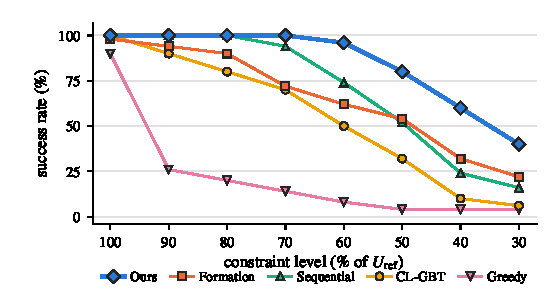
\includegraphics[width=\linewidth]{fig3a_success_vs_constraint}\\[-2pt]
  {\footnotesize (a)}\\[3pt]
  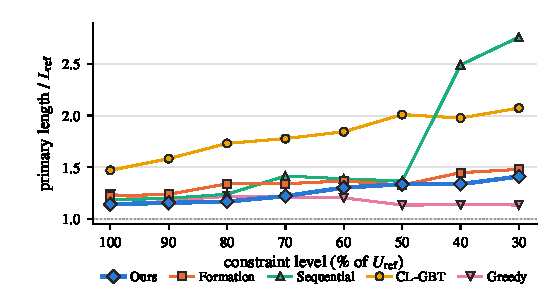
\includegraphics[width=\linewidth]{fig3b_length_vs_constraint}\\[-2pt]
  {\footnotesize (b)}
  \caption{Baseline comparison over the 50 randomized scenarios as the terminal
    uncertainty bound tightens from 100\% to 30\% of the single-agent reference
    $U_\mathrm{ref}$. (a)~Fraction of scenarios solved. (b)~Mean primary path
    length over the solved scenarios, normalized by the single-agent reference
    length $L_\mathrm{ref}$ (standard deviations in Table~\ref{tab:sweep}).
    Ours still solves 80\% of the scenarios at half the reference bound, at a
    mean cost of $1.34\,L_\mathrm{ref}$.}
  \label{fig:length_success}
\end{figure}

\begin{figure}[t]
  \centering
  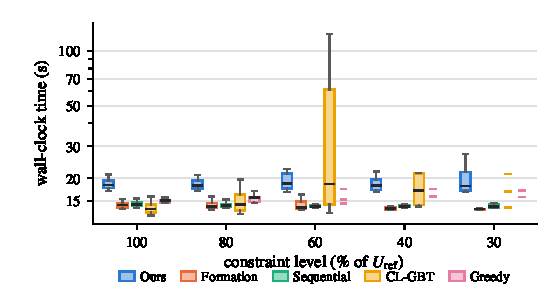
\includegraphics[width=\linewidth]{fig4_wall_5level_box}
  \caption{Wall-clock time per planner over successful runs, split by
    constraint level (log scale; five of the eight levels shown). Boxes span
    the interquartile range and whiskers extend to $1.5\times$ IQR; runs
    beyond the whiskers are omitted and the axis spans what remains, so the
    four planners that sit in 13--22\,s can be told apart. Only CL-GBT's
    search grows with the bound: at 60\% its upper quartile reaches 61\,s and
    its whisker 124\,s (its longest run took 730\,s). Where a planner solved
    fewer than five scenarios at a level there is nothing to summarize, so
    those runs are drawn individually, one tick each.}
  \label{fig:wall}
\end{figure}

Fig.~\ref{fig:length_success} reports the success rate and the path length
against the constraint level, and Table~\ref{tab:sweep} lists the lengths
with their spread across scenarios. Every planner but Greedy solves nearly
every scenario at the loosest level, where the bound equals the uncertainty
of the unconstrained reference, and the planners separate as the bound
tightens. Our planner solves every scenario down to 70\%, 96\% of them at
60\%, 80\% at 50\%, and 40\% at 30\%. Sequential matches it down to 80\% and
remains the strongest baseline at 70\% and 60\%, but falls to 52\% at 50\%
and 16\% at 30\%, and its solutions grow to more than twice the reference
length at the tightest levels, since at a tight bound the primary must
already detour to landmarks on its own before the support is planned.
Formation degrades more gracefully and is the strongest baseline from 50\%
down, with 54\% at half the reference bound and 22\% at 30\%. CL-GBT solves
half the scenarios at 60\% and 6\% at 30\%, with paths 1.5 to 2 times the
reference length at every level, since a rapidly exploring random tree
returns the first path it finds rather than the shortest. Greedy solves 90\%
at the loosest level and almost nothing below it, because a support that
cannot pay a detour now for a fix later rarely reaches a landmark in time.

The price of the higher success rate is modest. Our paths are the shortest
among the solved scenarios at every level, from $1.14\,L_\mathrm{ref}$ at
100\% to $1.41\,L_\mathrm{ref}$ at 30\%, and Table~\ref{tab:sweep} shows
that their spread across scenarios is also the smallest.
Fig.~\ref{fig:wall} reports the wall-clock time. Our planner takes a median
of 18\,s per run against 14\,s for Formation and Sequential and 16\,s for the
single-agent reference, and most of that time is fixed overhead shared by
every method. Only CL-GBT grows with the bound, since a tighter bound needs
a support placement that its sampler rarely proposes, and its longest run
took 730\,s.

\subsection{Ablation}

\begin{figure}[t]
  \centering
  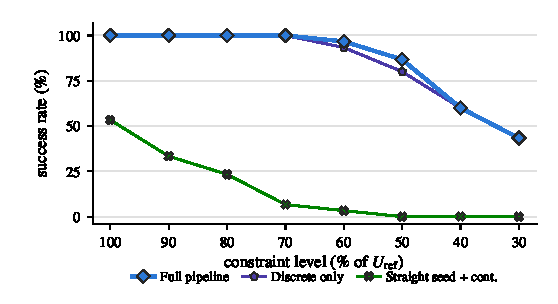
\includegraphics[width=\linewidth]{fig5a_abl_success_vs_constraint}\\[-2pt]
  {\footnotesize (a)}\\[3pt]
  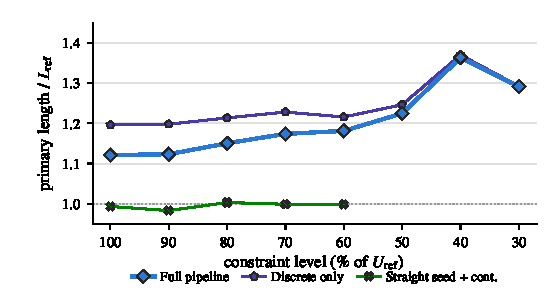
\includegraphics[width=\linewidth]{fig5b_abl_length_vs_constraint}\\[-2pt]
  {\footnotesize (b)}
  \caption{Ablation on a separate set of 30 randomized scenarios, drawn without
    the trivial-straight screen of Fig.~\ref{fig:length_success}, so the full
    pipeline is re-run on this set. Same axes as Fig.~\ref{fig:length_success}:
    (a)~success rate, (b)~mean path length over the solved scenarios (standard
    deviations in Table~\ref{tab:sweep}).
    The discrete stage alone solves the same scenarios as the full pipeline
    down to 70\% (the curves coincide) and slightly fewer at 60--50\%, with
    paths 2--7\% longer at every level down to 50\%, which is what the
    continuous refinement buys. Seeding the refinement from a straight line
    instead of the lattice solution solves only the scenarios where the
    straight run already meets the bound: half at 100\% and none below 60\%.}
  \label{fig:abl_length_success}
\end{figure}

\begin{figure}[t]
  \centering
  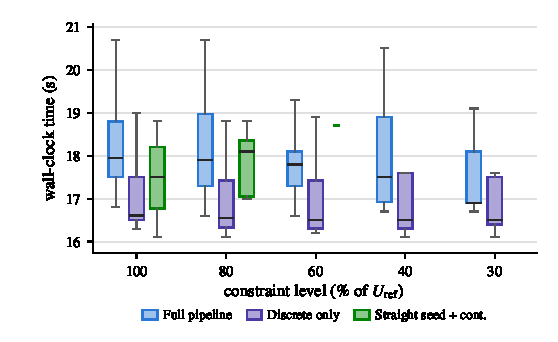
\includegraphics[width=\linewidth]{fig6_abl_wall_5level_box}
  \caption{Wall-clock time of the ablation arms over successful runs, split by
    constraint level and drawn as in Fig.~\ref{fig:wall} but on a linear axis:
    all three arms sit between 16 and 21\,s. The continuous refinement adds
    about 1.5\,s to the discrete stage. The straight-line seed skips the search
    yet costs the same as the full pipeline where it succeeds at all (its
    single run at 60\% is drawn as a tick).}
  \label{fig:abl_wall}
\end{figure}

\begin{table}[t]
  \caption{Mean $\pm$ SD of the primary path length over the solved scenarios,
    normalized by $L_\mathrm{ref}$, at four constraint levels (success rates
    are in Figs.~\ref{fig:length_success}a and~\ref{fig:abl_length_success}a).
    Top block: the 50 screened scenarios of
    Figs.~\ref{fig:length_success}--\ref{fig:wall}. Bottom block: the
    30-scenario ablation set of Figs.~\ref{fig:abl_length_success}--\ref{fig:abl_wall},
    on which the full pipeline is listed again. ``--'': no scenario solved.}
  \label{tab:sweep}
  \centering
  \footnotesize
  \setlength{\tabcolsep}{4pt}
  \begin{tabular}{@{}lcccc@{}}
    \toprule
    & \multicolumn{4}{c}{Constraint level (\% of $U_\mathrm{ref}$)} \\
    \cmidrule(l){2-5}
    Method & 100 & 70 & 50 & 30 \\
    \midrule
    Ours          & 1.14$\pm$0.09 & 1.22$\pm$0.23 & 1.34$\pm$0.26 & 1.41$\pm$0.21 \\
    Formation     & 1.22$\pm$0.12 & 1.34$\pm$0.25 & 1.33$\pm$0.16 & 1.48$\pm$0.45 \\
    Sequential    & 1.18$\pm$0.14 & 1.41$\pm$0.92 & 1.36$\pm$0.50 & 2.76$\pm$1.51 \\
    CL-GBT        & 1.47$\pm$0.33 & 1.78$\pm$0.43 & 2.01$\pm$0.41 & 2.07$\pm$0.26 \\
    Greedy        & 1.24$\pm$0.10 & 1.21$\pm$0.06 & 1.13$\pm$0.01 & 1.13$\pm$0.01 \\
    \midrule
    Full pipeline          & 1.12$\pm$0.14 & 1.17$\pm$0.23 & 1.22$\pm$0.22 & 1.29$\pm$0.22 \\
    Discrete only          & 1.20$\pm$0.15 & 1.23$\pm$0.23 & 1.25$\pm$0.22 & 1.29$\pm$0.22 \\
    Straight seed + cont.\ & 0.99$\pm$0.04 & 1.00$\pm$0.00 & -- & -- \\
    \bottomrule
  \end{tabular}
\end{table}

The ablation asks what each stage of the pipeline contributes. It runs on a
separate set of 30 scenarios drawn without the straight-line screen, since
one of the arms is the straight seed itself, and it compares the full
pipeline with the discrete stage alone and with the continuous refinement
seeded from a straight line. Fig.~\ref{fig:abl_length_success} and the
bottom block of Table~\ref{tab:sweep} report the results.

The discrete stage alone solves the same scenarios as the full pipeline down
to 70\% and one or two fewer at 60\% and 50\%. Its paths are 2 to 7\% longer
at every level down to 50\%, which is the length the refinement recovers by
cutting the lattice corners, and at the two tightest levels the two arms are
indistinguishable. The straight seed solves 53\% of the scenarios at the
loosest level and none below 60\%, and every solution it returns has a
length ratio of 1.00. The refinement therefore never found a feasible detour
from a straight seed and succeeded only where the straight line was feasible
to begin with. The joint search is what finds the landmarks, and the
refinement is what makes the route short. Fig.~\ref{fig:abl_wall} shows that
all three arms run in 16 to 21\,s, with the refinement adding about 1.5\,s to
the discrete stage.

% ===========================================================================
\section{SIMULATION VALIDATION}
% ===========================================================================
\budget{$\approx$700 words + 1 eq.\ + \cref{tab:noise}, 0.75 page of prose; floats
  Fig.~7, Fig.~8, \cref{tab:mc} add $\approx$0.55 page}
\todo{open with the purpose in one sentence: every planner in Sec.~V propagates
  the same covariance model, so the simulation is not a planner comparison ---
  it asks whether that model is \emph{calibrated} against a vehicle, controller
  and estimator that do not share its equations. Each plan is flown $N$ times
  with different noise seeds.}

\subsection{Simulator and Vehicle}
\budget{$\approx$150 words}
\todo{HoloOcean \todo{cite Potokar et al.\ (verify)}: 6-DOF Fossen AUV dynamics
  with the simulator's stock depth/heading autopilot at 30\,Hz; an outer-loop
  waypoint follower tracks the planned B-spline resampled every 25\,m (arrival
  radius 15\,m, set by the turn radius); the vehicle steers on the
  \emph{estimated} position, dead-reckoned forward between fixes. Three
  cadences, all scheduled on arc length accumulated from ground truth so that
  events land where the planner assumed them: control every tick, an estimator
  node every 5\,m, an acoustic comm every 100\,m (the planner's comm interval,
  range-gated with the planner's comm weight). Landmarks, obstacles, start and
  goal are imported from the plan; the 2-D field is lifted onto one depth plane.}
\lipsum[52]

\subsection{Factor-Graph State Estimator}
\budget{$\approx$350 words + \cref{eq:fg} + \cref{tab:noise}}
\todo{Credit: this is the collaborator's existing GTSAM \todo{cite GTSAM /
  iSAM2 (Kaess et al.), verify} stack, used essentially unchanged; say so.}
\todo{What it is (from \texttt{factor\_graph.py} / \texttt{main.py}):
  (a) iSAM2 incremental smoother over $SE(3)$ pose nodes, one node per 5\,m of
      arc, per agent;
  (b) \emph{anchor-node parameterization}: each agent estimates a local
      trajectory $\mathbf T^{\ell}_k$ plus an anchor $\mathbf T^{a}$, world pose
      $\mathbf T^{w}_k=\mathbf T^{a}\mathbf T^{\ell}_k$, Gaussian priors on both
      at deployment; the planner's 2-D $\Sigma$ corresponds to the $xy$ block of
      the \emph{world-pose} marginal;
  (c) two layers of graph: a per-agent dead-reckoning graph (own odometry
      between-factors, unary depth and 3-DOF orientation factors, and
      azimuth/elevation/range factors to landmarks within visibility range,
      each landmark carrying a prior with the planner's $\Sigma_\ell$ --- a
      known map, not SLAM) whose output is the relative pose and marginal the
      agent transmits acoustically; and the primary's multi-agent graph, which
      adds at every comm event the sender's compounded between-factor (its
      motion since the last comm, covariance $S_{jk}$) and an inter-agent
      acoustic bearing factor;
  (d) measurement synthesis: all measurements are ground truth from HoloOcean
      plus additive Gaussian noise (\cref{tab:noise}) --- no DVL/IMU sensor models;
      this tests the belief model's consistency, not sensor realism (say so,
      and repeat in Sec.~VII).}
\todo{OPEN --- write this against what is actually flown for the final numbers.
  Pending in \texttt{multiagent\_base/ESTIMATOR\_REVIEW.md}: E1 report the
  world-pose marginal, not the anchor-relative local one; E2 the inter-agent
  factor is bearing-only today while the planner models a range-gated
  position transfer (CI) --- either land the relative-position factor or
  state the mismatch as a limitation; E3 path for a support's landmark fix
  into the primary's graph; E4 transmitted-covariance bookkeeping; E6 noise
  parameters calibrated to the planner's dead-reckoning rates (plan A2--A4).}
\begin{equation}
  \hat{\mathcal X}=\arg\min_{\mathcal X}\;\sum_{i\in\mathcal F}
    \big\lVert r_i(\mathcal X)\big\rVert^{2}_{\Sigma_i},
  \qquad
  \mathbf T^{w}_{k}=\mathbf T^{a}\,\mathbf T^{\ell}_{k}
  \label{eq:fg}
\end{equation}

\begin{table}[t]
  \caption{Factor noise of the simulated estimator, derived from the planner's
    noise model so that both codebases share one ruler: along-track odometry
    from $q_\parallel$, the compass from $q_\perp$, landmark noise from the
    planner's per-pass value rescaled to one sighting per 5\,m node, and
    communication noise $\sigma_c$ divided by $\sqrt{w}$ for link weight $w$.
    Poses are estimated in the world frame; the prior on the known start pose
    carries the planner's $\Sigma^0$ in $x$, $y$.
    \todo{the depth factor $\sigma$ (0.5\,m) still differs from the injected
    depth noise (0.01\,m); not re-verified}}
  \label{tab:noise}
  \centering
  \scriptsize
  \setlength{\tabcolsep}{3pt}
  \begin{tabular}{@{}llc@{}}
    \toprule
    Factor & Variables & $\sigma$ \\
    \midrule
    Odometry (between, per 5\,m node) & $\mathbf T_{k-1},\mathbf T_k$ & 1$^\circ$/axis; 0.22, 0.02, 0.01\,m \\
    Depth (unary) & $\mathbf T_k$ & 0.5\,m \\
    Compass (unary) & $\mathbf T_k$ & 0.86$^\circ$/axis \\
    Landmark az./el./range & $\mathbf T_k,\ell$ & 1.05$^\circ$, 1.05$^\circ$, 2.09\,m; $r<100$\,m \\
    Inter-agent relative pose & $\mathbf T^{s}_k,\mathbf T^{p}_k$ & 0.86$^\circ$/axis; $0.5/\sqrt{w}$\,m \\
    Initial pose prior & $\mathbf T_0$ & 10$^\circ$/axis; 1.15, 0.76, 0.5\,m \\
    \bottomrule
  \end{tabular}
\end{table}
\lipsum[54]

\subsection{Monte Carlo Results}
\budget{$\approx$200 words; Fig.~7, Fig.~8 and \cref{tab:mc} live here}
\todo{report per trial: goal reached, obstacle penetration vs.\ the
  allocated $\Delta$, terminal $\det(\Sigma)^{1/4}$ predicted vs.\ empirical
  (planner model on the flown track vs.\ estimator marginal vs.\ sample
  covariance of the true error); one sentence on why baselines are not
  re-flown (shared belief model, see Sec.~VII)}

\begin{figure}[t]
  \centering
  \figbox{4cm}{Fig.~7 --- HoloOcean screenshot: what the simulated
    environment looks like}
  \caption{The HoloOcean \todo{cite} environment used for validation.
    \todo{write real caption}}
  \label{fig:holoocean}
\end{figure}

\begin{figure}[t]
  \centering
  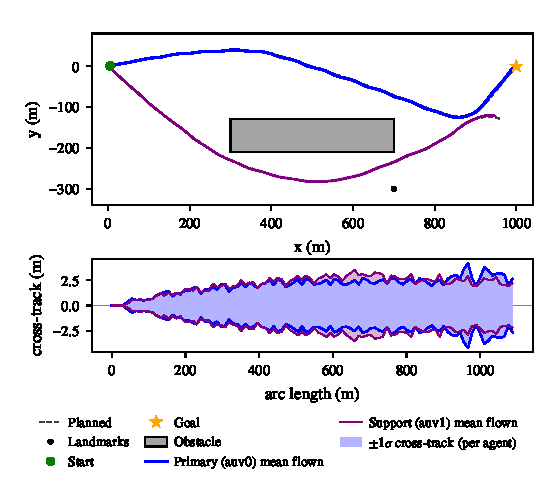
\includegraphics[width=\linewidth]{fig8_mc_behind_wall}
  \caption{Closed-loop Monte Carlo of the behind-wall plan in HoloOcean, 30
    runs with different noise seeds: planned trajectories (dashed) against the
    mean executed trajectory of each agent, with the $\pm2\sigma$ cross-track
    envelope of the runs drawn on the map. The primary passes north of the
    obstacle while the support diverts south to the landmark and rejoins before
    the goal. The $2\sigma$ half-width is about 4\,m along the 1.1\,km route
    and peaks at 8\,m on the primary's final bend; every run reaches the goal
    and clears the obstacle.}
  \label{fig:mc_paths}
\end{figure}

\begin{table}[t]
  \caption{Monte Carlo constraint satisfaction in HoloOcean: the behind-wall
    plan of Fig.~\ref{fig:mc_paths} (two agents, one obstacle, one landmark,
    $\bar u = 1.8$\,m) flown 30 times with different noise seeds. Collision
    rate counts runs with any obstacle penetration, against the allocated
    $\Delta = PM\delta = 0.10$; the terminal bound is met when the estimator's
    marginal at the goal is under $\bar u$; $\sigma_T$ is the planner's
    prediction against the sample covariance of the true terminal error over
    the runs.}
  \label{tab:mc}
  \centering
  \footnotesize
  \setlength{\tabcolsep}{4pt}
  \begin{tabular}{@{}lcccc@{}}
    \toprule
    Case & Runs & \makecell{Collision\\rate ($\le\Delta$)} & \makecell{Terminal\\bound met} & \makecell{Pred.\,/\,emp.\\$\sigma_T$} \\
    \midrule
    Behind wall & 30 & 0/30 & 28/30 & 1.80\,/\,1.70 \\
    \bottomrule
  \end{tabular}
\end{table}

\lipsum[44]

% ===========================================================================
\section{DISCUSSION AND LIMITATIONS}
% ===========================================================================
\budget{$\approx$400 words, 0.4 page}
\todo{cover, roughly one paragraph each:
  (i) discretization and completeness --- replaces the old optimality
      guarantee: the lattice phase is exogenous to obstacle geometry, so the
      discrete feasible set is neither a subset nor a superset of the true one,
      and refinement cannot rescue it;
  (ii) Gaussian belief + maximum-likelihood-observation assumption
      (platt2010belief) --- the simulation validation is what tests whether it
      is calibrated;
  (iii) centralized, offline, open-loop plan; replanning not addressed;
  (iv) cost: 1.3--1.9$\times$ the reference wall clock; Floyd--Warshall
      $O(n^3)$ bounds the graph; joint space exponential in agents, two tested;
  (v) 2-D, static, convex obstacles with known $\Sigma_o$;
  (vi) why the baselines are not re-run in simulation (shared belief model);
  (vii) simulated measurements are ground truth plus Gaussian noise ---
      the simulation tests belief-model consistency, not sensor realism.}

\lipsum[47]

% ===========================================================================
\section{CONCLUSION}
% ===========================================================================
\budget{$\approx$150 words, 0.15 page}

\lipsum[51]

% DRAFT: \nocite{*} makes the bibliography non-empty so its height is counted.
% Remove it once the text carries real \cite commands.
\nocite{*}
\bibliographystyle{IEEEtran}
\bibliography{refs}

\end{document}
